\documentclass[border=10pt]{standalone}

\usepackage[utf8]{inputenc}
\usepackage[english]{babel}
\usepackage{tikz}
\usetikzlibrary{decorations.text}
\usetikzlibrary{positioning, arrows.meta, fit}
\usepackage{tkz-graph}	
\usetikzlibrary{automata,arrows}
\usetikzlibrary{calc}

\begin{document}
	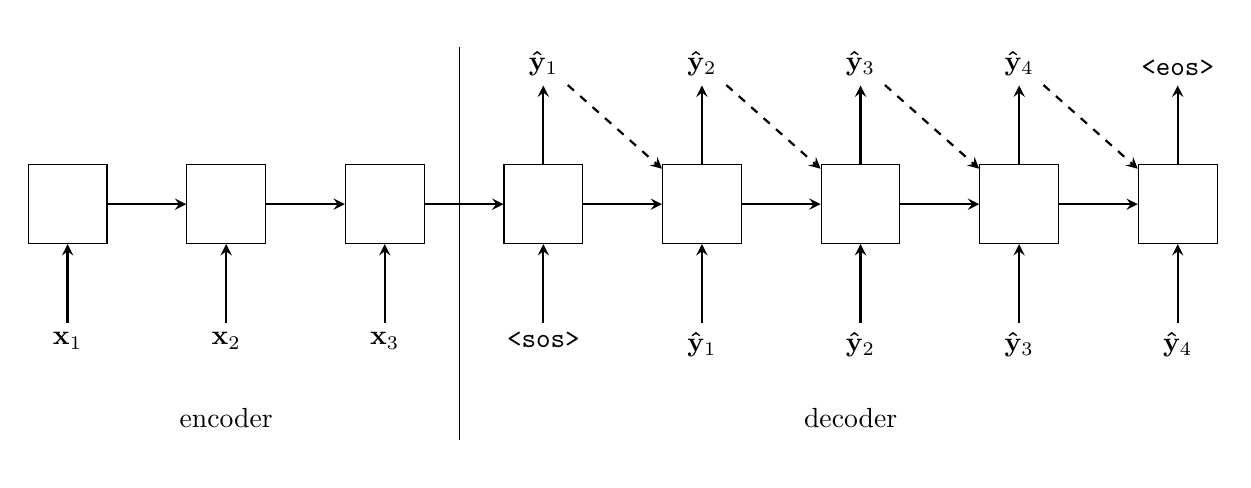
\begin{tikzpicture}
		% seq2seq layer
		\node[rectangle, draw, minimum height=1cm, minimum width=1cm] (al11) {};
		\node[rectangle, right=of al11, draw, minimum height=1cm, minimum width=1cm] (al12) {};
		\node[rectangle, right=of al12, draw, minimum height=1cm, minimum width=1cm] (al13) {};
		\node[rectangle, right=of al13, draw, minimum height=1cm, minimum width=1cm] (al21) {};
		\node[rectangle, right=of al21, draw, minimum height=1cm, minimum width=1cm] (al22) {};
		% separation line between encoder decoder
		\node[above=2cm of al13] (upp) at ($(al13)!0.5!(al21)$) {};
		\node[below=3cm of al13] (bel) at ($(al13)!0.5!(al21)$) {};
		\draw[transform canvas={xshift=-1.5pt}] (upp) -- (bel);
		\node[rectangle, right=of al22, draw, minimum height=1cm, minimum width=1cm] (al23) {};
		\node[rectangle, right=of al23, draw, minimum height=1cm, minimum width=1cm] (al24) {};
		\node[rectangle, right=of al24, draw, minimum height=1cm, minimum width=1cm] (al25) {};
		% inputs - encoder
		\node[below=of al11] (X1) {$\mathbf{x}_{1}$};
		\node[below=of al12] (X2) {$\mathbf{x}_{2}$};
		\node[below=0.5cm of X2] (enc) {$\textnormal{encoder}$};
		\node[below=of al13] (X3) {$\mathbf{x}_{3}$};
		\node[below=of al21] (y0) {$ \texttt{<sos>}$};
		% inputs - decoder
		\node[below=of al22] (y1d) {$\mathbf{\hat{y}}_{1}$};
		\node[below=of al23] (y2d) {$\mathbf{\hat{y}}_{2}$};
		\node[right=6.5cm of enc] (dec) {$\textnormal{decoder}$};
		\node[below=of al24] (y3d) {$\mathbf{\hat{y}}_{3}$};
		\node[below=of al25] (y4d) {$\mathbf{\hat{y}}_{4}$};	
		% outputs
		\node[above=of al21] (y1) {$\mathbf{\hat{y}}_{1}$};
		\draw[-stealth, dashed, thick] (y1) -- (al22);
		\node[above=of al22] (y2) {$\mathbf{\hat{y}}_{2}$};
		\draw[-stealth, dashed, thick] (y2) -- (al23);
		\node[above=of al23] (y3) {$\mathbf{\hat{y}}_{3}$};
		\draw[-stealth, dashed, thick] (y3) -- (al24);
		\node[above=of al24] (y4) {$\mathbf{\hat{y}}_{4}$};
		\draw[-stealth, dashed, thick] (y4) -- (al25);
		\node[above=of al25] (y5) {$ \texttt{<eos>}$};
		% forward input arrows - encoder
		\draw[-stealth, thick] (X1) -- (al11);
		\draw[-stealth, thick] (X2) -- (al12);
		\draw[-stealth, thick] (X3) -- (al13);
		\draw[-stealth, thick] (y0) -- (al21);
		% forward input arrows - decoder
		\draw[-stealth, thick] (y1d) -- (al22);
		\draw[-stealth, thick] (y2d) -- (al23);
		\draw[-stealth, thick] (y3d) -- (al24);
		\draw[-stealth, thick] (y4d) -- (al25);
		% forward output arrows
		\draw[-stealth, thick] (al21) -- (y1);
		\draw[-stealth, thick] (al22) -- (y2);
		\draw[-stealth, thick] (al23) -- (y3);
		\draw[-stealth, thick] (al24) -- (y4);
		\draw[-stealth, thick] (al25) -- (y5);
		% forward hidden states
		\draw[-stealth, thick] (al11) -- node[above, pos=0.35] {} (al12);
		\draw[-stealth, thick] (al12) -- node[above, pos=0.35] {} (al13);
		\draw[-stealth, thick] (al13) -- node[above, pos=0.35] {} (al21);
		\draw[-stealth, thick] (al21) -- node[above, pos=0.35] {} (al22);
		\draw[-stealth, thick] (al22) -- node[above, pos=0.35] {} (al23);
		\draw[-stealth, thick] (al23) -- node[above, pos=0.35] {} (al24);
		\draw[-stealth, thick] (al24) -- node[above, pos=0.35] {} (al25);
	\end{tikzpicture}
\end{document}